\chapter{Facebook Privacy}
\label{chp:defaultprivacysettings} 

In this chapter we are going to look into was kind of privacy settings that exist on Facebook. We will also look at and map how the default privacy settings has evolved over time. In addition to this we will look at some of the features introduced by Facebook over the years, and how these features have effected the privacy on Facebook. Finally we will review some of Mark Zuckerberg's  thoughts and comments in regard to Facebook privacy. 


\section{Privacy on Facebook}\label{sec:privacy_on_facebook}

\begin{figure}[h!]
\centering
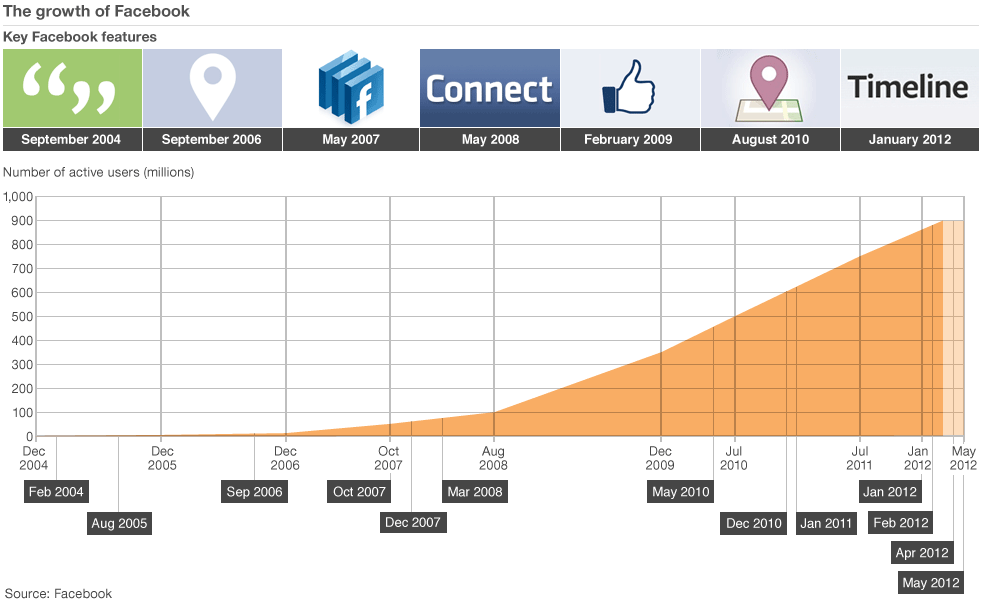
\includegraphics[width=0.8\textwidth]{gowth_of_facebook.png}
\caption[The development of Facebook users and introduction of new features]{\textbf{The development of Facebook users and introduction of new features.} The orange field in the graph shows the increasing number of Facebook users over the years. Key Facebook features are shown over the graph according to when they were introduced \cite{BBCFacebookGrowth}.} 
\label{fig:growth_of_facebook}
\end{figure}

There is no doubt that Facebook has had a remarkable development, both when it comes to number of active users and the development of new features, as shown in \fref{fig:growth_of_facebook}. Along with new users and new features, there has also been made major changes to what kind of privacy settings exists and what kind are needed. 


\subsection{Facebook Settings}
Whenever Facebook make an update to the settings, the users usually get a personal message informing them about the change. Because of the high number of users, this change happens gradually. This means that not everyone will get a notification about the changes made at once \cite{settingschangingagain}. Despite the changes over time, the main control of ones privacy lies in the hands of the users. The users have the opportunity to make their profile more secure, than what is set to default. 

\subsubsection{The settings that exists}
There exists numerous settings one can edit to make the profile more or less secure. The main problem here is probably that many people are not aware of these settings, or are not confident enough in changing them. Regardless of this the settings exists, and it is up to each one of the users how they could be configured. 
On the Facebook settings page you have different tabs regarding different kind of settings. These settings available are elaborated in \tref{tab:settings}.

\newpage

\begin{center}
    \begin{longtable}{ | l | p{9cm} |}
    \caption{\label{tab:settings}The settings that exist on Facebook 				\cite{facebooksettings}.} \\
    \hline
    \textbf{Setting tab} & \textbf{Description} \\ 
    \hline
    General & Under this tab you can edit your name, username, email, \textit{password}, which network you are in and language. \\
    \hline
    Security & Under this tab you can do changes that makes it harder for someone else to hack into your Facebook account. Here you can enable/disable \textbf{Secure Browsing} (the use of https when possible). It is possible to turn on \textbf{Login Notification}. This means you will get notified either by email or text message (after you choice) when your account is accessed from a computer or mobile device that you haven't used before. You can also enable something called \textbf{Login Approvals}, where a security code is required to access your account from a unknown browser. This code can be given to you in a text message sent to your mobile. You also have the chose to use \textbf{Code Generator} on your Facebook mobile app to reset your password or generate login approvals security codes. Under the security tab you can also create \textbf{App Passwords}, add \textbf{Trusted Contacts}, view \textbf{Recognized Devices} and \textbf{Active Sessions}. Under active sessions you can see all sessions active via your accout. Here you can look for unfamiliar devices or locations, and if you find a session that is not you, someone else have been logged into your account. This session can easily be ended. \\ 
    \hline
    Privacy & Under this tab you can change the audience for your future posts You can also chose who can send you friend requests, who can look you up using the email address you provided and who can look you up using the phone number you provided. The last setting concerns whether or not you want other search engines to link to your timeline. This can either be turned On or Off.\\
    \hline
    Timeline and Tagging & Under this tab you can chose who can post on your timeline, who can see posts you've been tagged in on your timeline and who can see what others post on your timeline. You can also choose whether or not you want to review tags people add to your own posts before the tags appear on Facebook, and you can choose the audience for a post you're tagged in if they aren't already in it.\\
	\hline
    Blocking & Under this tab you can block users, app invites from specific users, event invites and specific apps. Under this tab you can also make a \textbf{Restricted List}. Your friends on this list will only be able to see the information and posts that are public.\\
    \hline
    Notifications & Under this tab you can control how you get notifications, and what you get notified about.\\
    \hline
    Mobile & Under this tab you can add your phone number(s), and activate registered phone(s) for text messaging.\\
    \hline
    Followers & Under this tab you can turn on follow, this makes it possible for other people to follow you. Followers will only see your public posts and will not be added as friends.\\
    \hline
    Apps & Here you can choose whether or not you want to use apps, games and websites on Facebook and elsewhere. You also get a list of the apps you use, and you can edit the audience for things posted via these apps. The people on Facebook who can see your information can bring this information with them when they use apps. This is to improve the user experience. Under \textbf{Apps other use} you can control the categories of information that people can bring with them when they use apps, games and websites. You can also turn on something called \textbf{Instant personalization}, which let you see relevant information about your friends the moments you arrive on select partner websites. Finally, under this tab you can choose the audience for the things posted using old Facebook mobile apps that do not have the in-line audience selector.\\ 
    \hline
    \end{longtable}
\end{center}



\section{Default Settings on Facebook}\label{sec:default_privacy_settings}

Facebook has evolved from being a networking site for students attending Harvard to becoming a global phenomenon. Facebook's user interface has gone through several changes over the years, which has brought both joy and frustration to the users. When these changes have been made, there has also been adjustments to the default privacy settings as well \cite{EvoPriv2}. At the beginning, in 2005, when Facebook first was applied outside of Harvard University, the users personal information was only accessible to a users Facebook friends and to people connected to the same network on Facebook \cite{EvoPriv}. This is far from reality today. We will now look into how the default privacy settings on Facebook has developed over since it was first introduced. 


\subsection{Development of Default Settings}

%- skrive litt mer her, en slags intro


%- utdype tabellen 

The main changes to the default privacy settings are emphasized in\begin{center}
\begin{table}[!ht]
\caption{\label{tab:dps}Changes in the default privacy settings on Facebook from 2005 until today. \cite{EvoPriv,PrivTimeline}}
    \begin{tabular}{ | l | p{9cm} |}
    \hline
    \textbf{Year} & \textbf{Default Privacy Settings} \\ 
    \hline
    2005 & Personal information (e.g., name and profile picture) is 	only visible to specific groups specified in your privacy 			settings.\\ 
    \hline
    2006 & The only information displayed in your profile is your 		school and specified local area. \\ 
    \hline
    2007 & Name, name of school (network) and profile picture 			(thumbnail) is available to all Facebook users.\\
    \hline
    November 2009 & Name, profile picture and demographics is 			available and searchable to the entire Internet. In addition to 	this, list of friends are visible to all Facebook users.\\
	\hline
    December 2009 & Your name, profile picture, list of friends, 		pages you are fan of, demographics and likes are available for 		the entire Internet.\\
    \hline
    April 2010 & The entire Internet can see everything, except 		wall posts that are limited to friends and photos that are 			limited to your network. \\
    \hline
    2011 &  \\
    \hline
    2012 & \\
    \hline
    November 2013 & The entire Internet can see everything, except posts you've been tagged in on your timeline and others posts on your timeline, which are limited to friends of friends. \\ 
    \hline
    \end{tabular}
   \end{table}
\end{center} \tref{tab:dps}. 

% utdype mer, se kilde
Secure browsing became default in July 2013. Since 2011 users have been able to turn on secure browsing.  \cite{secureBrowsing}

\subsection{Default Settings 2013}
\label{subsec:default2013}

To examine the default settings on Facebook anno 2013, we created a new Facebook profile, so we could see how the settings were as default. \fref{fig:security2013}, \fref{fig:privacy2013}, \fref{fig:timelineandtagging2013} and \fref{fig:apps2013} shows the outline of the different settings without any alterations, in other words the default settings. 

\fref{fig:security2013} shows how the default security settings look like in November 2013. As we can see from the Figure, secure browsing is enabled by default. 

\begin{figure}[h!]
\centering
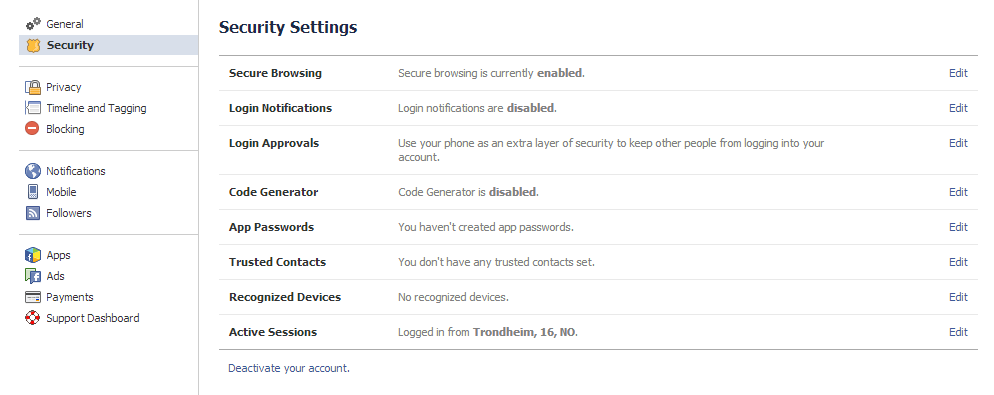
\includegraphics[width=1\textwidth]{default_nov_2013_security.png}
\caption[Default security settings on Facebook November 2013]{\textbf{Default security settings on Facebook November 2013}. This Figure shows the default security settings on Facebook in November 2013.} 
\label{fig:security2013}
\end{figure}

\begin{figure}[h!]
\centering
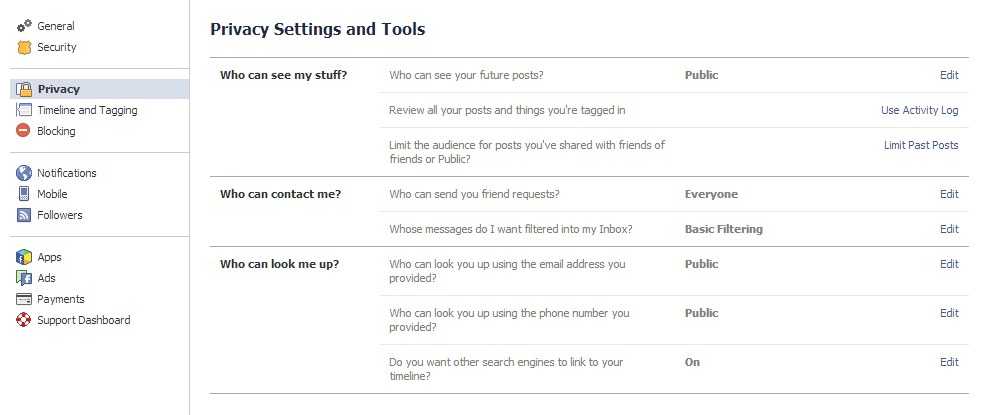
\includegraphics[width=1\textwidth]{default_nov_2013_privacy.png}
\caption[Default privacy settings on Facebook November 2013]{\textbf{Default privacy settings on Facebook November 2013}. This Figure shows the default privacy settings on Facebook in November 2013.} 
\label{fig:privacy2013}
\end{figure}

\begin{figure}[h!]
\centering
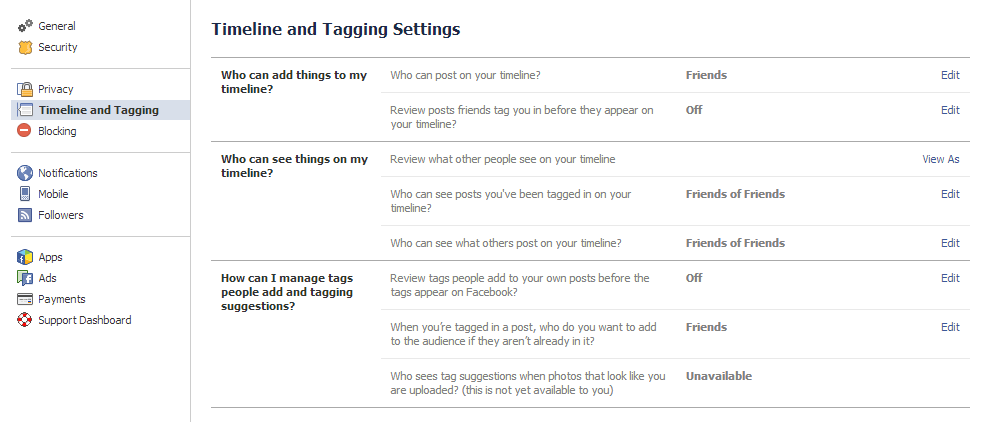
\includegraphics[width=1\textwidth]{default_nov_2013_timelineandtagging.png}
\caption[Default settings for timeline and tagging on Facebook November 2013]{\textbf{Default settings for timeline and tagging on Facebook November 2013}. This Figure shows the default settings for timeline and tagging on Facebook in November 2013.} 
\label{fig:timelineandtagging2013}
\end{figure}

\begin{figure}[h!]
\centering
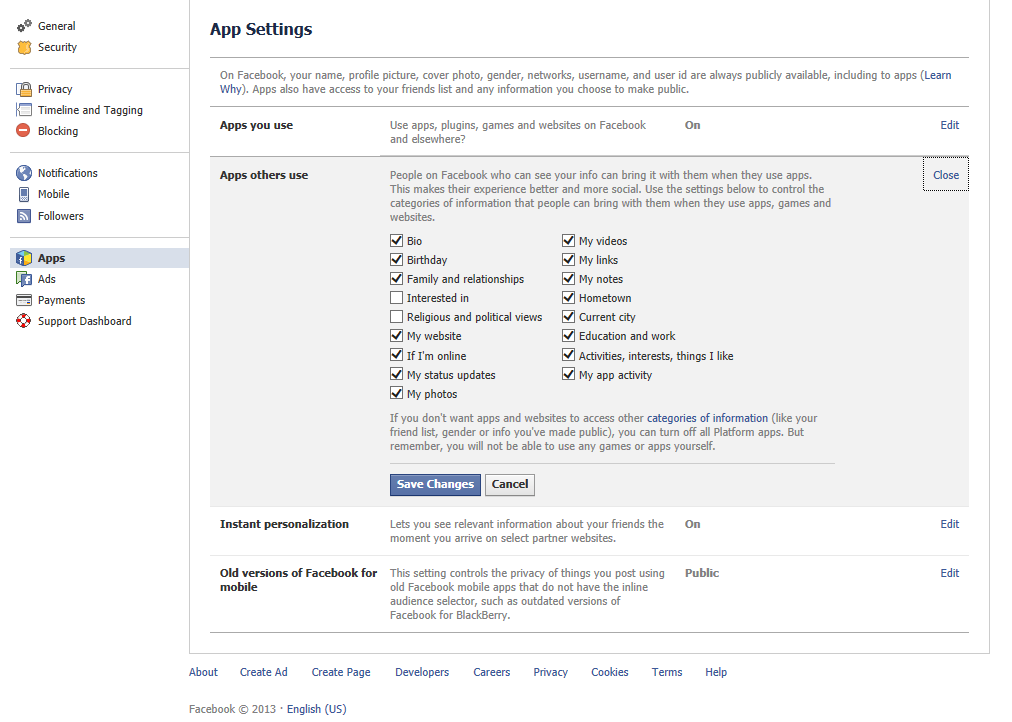
\includegraphics[width=1\textwidth]{default_nov_2013_apps.png}
\caption[Default settings for apps on Facebook November 2013]{\textbf{Default  settings for apps on Facebook November 2013}. This Figure shows the default settings for applications on Facebook in November 2013.} 
\label{fig:apps2013}
\end{figure}

\fref{fig:privacy2013} shows the default privacy settings in November 2013.  \textit{"Who can see your future posts?"} is set to \textit{Public}, which means everyone can view you posts. \textit{"Who can send you friend requests?"} is set to \textit{Everyone}. \textit{"Who can look you up using the email address you provided?"} and \textit{"Who can look you up using the phone number you provided?"} is set to \textit{Public}, which means it is easier for people to find you on Facebook if they know you email or phone number. The setting \textit{"Do you want other search engines to link to your timeline?"} is turned \textit{on}. This means that for example if you google a person, the Facebook profile will appear in the search. To summarize, the privacy settings are \textit{as public as they can get} by default. 

\fref{fig:timelineandtagging2013} shows the default settings for timeline and tagging on Facebook in November 2013. \textit{"Who can post on your timeline?"} is set to \textit{Friends}, which means that only Facebook friends can add things to your timeline. \textit{"Review posts friends tag you in before they appear on your timeline?" }is set to\textit{ off}. This means when friends tags you in something, it will appear on your timeline before you have had a chance to review it. In most cases this is probably fine, but it may occur that a Facebook friends tag you in something you would not prefer to have displayed on your timeline. In these cases it would be desirable to have the review-setting turned on. \textit{"Who can see posts you've been tagged in on your timeline?"} and \textit{"Who can see that others post on your timeline?"} is set to \textit{Friends of Friends}. In contrary to those who can post on your timeline, which are friends, friends of friends are able to view the content added to your timeline. If you have many friends on Facebook, and these friends have many friends each, the audience for posts are suddenly extremely large. 

\fref{fig:apps2013} shows the default settings for apps on Facebook in November 2013. Usage of apps, plugins, games and websites on Facebook and elsewhere are turned on by default. Under "Apps others use" you can choose which categories of information that people can bring with them when they use apps, games and websites. As you can see in the figure, almost every box i checked as default. The only exception is "Interested in" and "Religious and political views". As also shows in the figure, instant personalization is enabled by default and the privacy settings for the information you post/have posted using old Facebook mobile apps is set to public as default. 

\paragraph{Default settings does not preserve privacy} It is safe to conclude that the default privacy settings on Facebook anno 2013 is far too public. Unless there are conducted changes to the privacy settings, the timeline will be publicly available, with the exception of posts you've been tagged in and other's posts on your timeline which is "only" visible to friends, and friends of friends. 

\subsection{Default Settings for Teens}

\begin{figure}[h!]
\centering
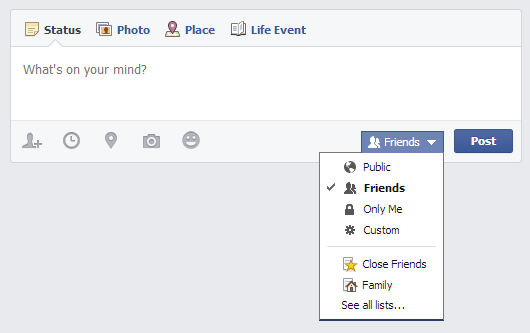
\includegraphics[width=0.8\textwidth]{new_post.png}
\caption[Choosing who can see a status update.]{\textbf{Choosing who can see a status update}. When posting a new post the user can choose the audience the post will be visible to. This can either be "public", "friends", "only me" or "custom".} 
\label{fig:newPost}
\end{figure}

\begin{figure}[h!]
\centering
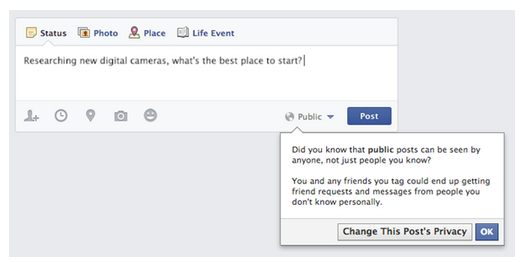
\includegraphics[width=0.8\textwidth]{teensSharePost.png}
\caption[The message shown to teens when posting to the public for the first time]{\textbf{The message shown to teens when posting to the public for the first time.} After the first time they post to the public the message in \fref{fig:sharePost} is shown \cite{defaultTeens}.} 
\label{fig:teensSharePost}
\end{figure}

\begin{figure}[h!]
\centering
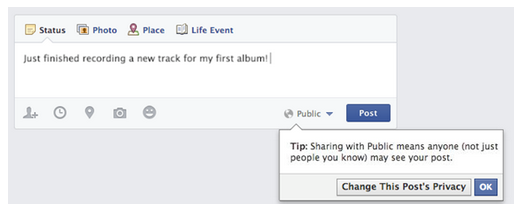
\includegraphics[width=0.8\textwidth]{sharePost.png}
\caption [The message shown to teens when posting to the public, except for the first time]{\textbf{The message shown to teens when posting to the public, except for the first time.} The first time they post to the public the message in \fref{fig:teensSharePost} is shown \cite{defaultTeens}.} 
\label{fig:sharePost}
\end{figure}

Each time a user on Facebook share a status update, the user chooses who the post is visible to, see \fref{fig:newPost}. The change you make will remain the same in future posts, unless you decide to change it. Up until today the default audience is set to "public", but for teens between 13-17 years, it has been "friends of friends". On October 16th Facebook announced to change the default setting for teens \cite{defaultTeens}. Now the initial audience for posts are "friends". Teens can later change this to "public", this was not a option before. Teens are active users of social media, and have want to be heard, either it is political engagement or an opinion on a movie. Further Facebook allows teens to turn on Follow, by doing this their public posts will show up in people's news feeds. Facebook designed these changes to improve the facebook experience for young people. In \cite{defaultTeens} Facebook also makes it clear that they take the safety of teens very seriously, and therefore have created a more extensive warning message, shown in  \fref{fig:teensSharePost}. This message appears when a teen changes the audience for their post. If they continue to post to the public, they will will get an additional reminder message, as shown in  \fref{fig:sharePost}.

\section{Facebook Features - Impact on your Privacy}\label{sec:facebook_features}

\subsection{News Feed}
\paragraph{}
News Feed is the first thing you see when you log into your Facebook account. It is a list that constantly is updated. This list includes the activity from your friends and info about Pages you follow on Facebook. Examples of activities that are shown on the News Feed are photos, status updates, links, apps, likes, comments, posts written on timelines and so on. Often are activities with many comments or likes on top of your News Feed. The reason for this is that Facebook uses a algorithm to determine "top stories". The algorithm takes several elements into account when deciding top stories; number of comments, who posted it, and what kind of post it is. The users also have the opportunity to filter their News Feed to for example activity just from close friends, most recent activities, activities of the users in a same network etc. \cite{newsfeed}.

When News Feed was introduced in 2006, many users showed disapproval because they was not given the control of who could see their updates, and was not able to opt out. A consequence of this disapproval was the creation of a group called "Students Against Facebook News Feed", which got 300 000 members in two days. This lead to an apologize by Zuckerburg: "We really messed this one up. We didn't build in the proper privacy controls". He stated that this was a big mistake on their part \cite{newsfeed2}. 


\subsection{Facebook Platform - Apps}
\label{subsec:app}
The Facebook Platform was launched in May 2007 at a developers conference in San Fransisco. This feature enabled a third-party developer to build social applications \cite{BBCFacebookGrowth}. These applications will then be integrated with Facebbok, both mobile and on the web. “Right now, social networks are closed platforms,” Zuckerberg said. “And today, we’re going to end that” \cite{platformStory}. Zuckerburg promised the developers a level playing field, and the opportunity to build apps that could compete with the ones Facebook created themselves. As well as access to the network's at that time 24 million users. In \cite{platformStory} McKenzie talk about the launching moment as the moment when Facebook transitioned from having MySpace as a competitor, to getting Google as the competitor. And that Facebook went from being a wall to start being a platform. 

18 months after it was launched, Facebook had abandoned the idea of a level playing field, and had started baking in features that cut of developers who tried to develop similar products as Facebook. Terms as "Zucked over" became more normal amongst developers. What was once looked at as a beautiful piece of engineering, had became a disappointment. Today the platform is mainly used to distribute games. Zynga, who made popular games like Farmville, is about the only company who have managed to build their whole business inside the Facebook Platform. The platform did not become what it intended, and as big as everybody was hoping for. And according to Facebook's own developers it has been a hard one to swallow. 

Even though Platform did not reach out to all the areas originally intended, it is still popular. By the the end of March 2012, there are more than 9 million apps and websites integrated with Facebook through the platform \cite{fbPlatform}.

As mentioned in section \ref{sec:intpriv}, apps are one area that highly concerns the users to interdependent privacy. Facebook Help Center \cite{faceHelp} explains that apps are designed to enhance the user experience with engaging games and useful features. In order for the apps to do this they ask you to share personal information. All apps ask for your basic information, this consists of your name, profile picture, cover photo, gender, networks, username, and user id. This is information that always is publicly available. Apps also have access to your friends list and any information you choose to make public. The apps ask for this information to enhance the users experience by personalising content, helping the user find friends that also uses the app, and make sharing of information easier. As well as speeding up the sign-up process, so that the user can start using the game or app right away. 

\paragraph{Application permissions.} As of November 2013 Facebook has 54 permissions divided into 6 different categories \cite{permission}. These categories are email, permissions, extended, extended profile properties, open graph permissions, page permissions and public profile and friend list. 

\paragraph{Apps privacy control.}In the Facebook settings \cite{facebooksettings} under the tap "Apps" the user can manage apps, \fref{fig:apps2013}, and control what information that will be shared with apps others use. The user also has the opportunity to turn off all platform applications. The user will then no longer be able to use any games or other applications.

\subsubsection{Installing an Application}
We will now look at the process of installing an application from Facebook Platform. As mentioned when installing an app, the user will be asked to give permissions to share information. This information vary a lot, some just ask for your basic information, some ask for relationship status, birthday and also permission to post to your Timeline in your name. We have looked at the very popular application TripAdvisor. According to the site secure.me \cite{secure.me} TripAdvisor have a poor reputation because it may be a treat to your privacy.  

\paragraph{Installing on a PC.}
When opening TripAdvisor in Facebooks App Center on a personal computer, we are directed to TripAdvisors page, as shown in \fref{fig:tripadvisorpc}. The page contains information about the application, as well as the permissions required. These permissions are shown in the top right corner. The permissions that TripAdvisor requires exceeds beyond on basic information. We can put these permissions in the follwing privacy groups; personal privacy, relational privacy and spatial privacy. Personal privacy contains the permissions to access personal information about the user like location, education, hometown, work history, your photos, your status updates, e-mail address and likes. Relational privacy includes retrieving friends' profile information; education history, hometown, likes, locations and work history. As well as photos shared with you, and status updates shared with you. The last privacy category, spatial privacy, concerns posts that the app post on your behalf on your Timeline. By default these posts are set to public, but you can easily change the setting before installing the app. When pushing the "Go to App"- button, you automatically give your consent to required permissions and install the App. this can be misleading, since the user might look for a installation button, or some kind of verification that the installation has started. This may lead to an app being installed without the user knowing. The permissions are all shown, and explained, but not as visible as they used to be before App Center was introduced. \fref{fig:permissions2011} shows the authentication dialogue as of 2011, before App Center was introduced. You got a pop-up windows stating all the permissions requested by the app. The use of pop-up windows like these made it much easier for the user to review the permissions, and to not miss out on them. 

\begin{figure}[h!]
\centering
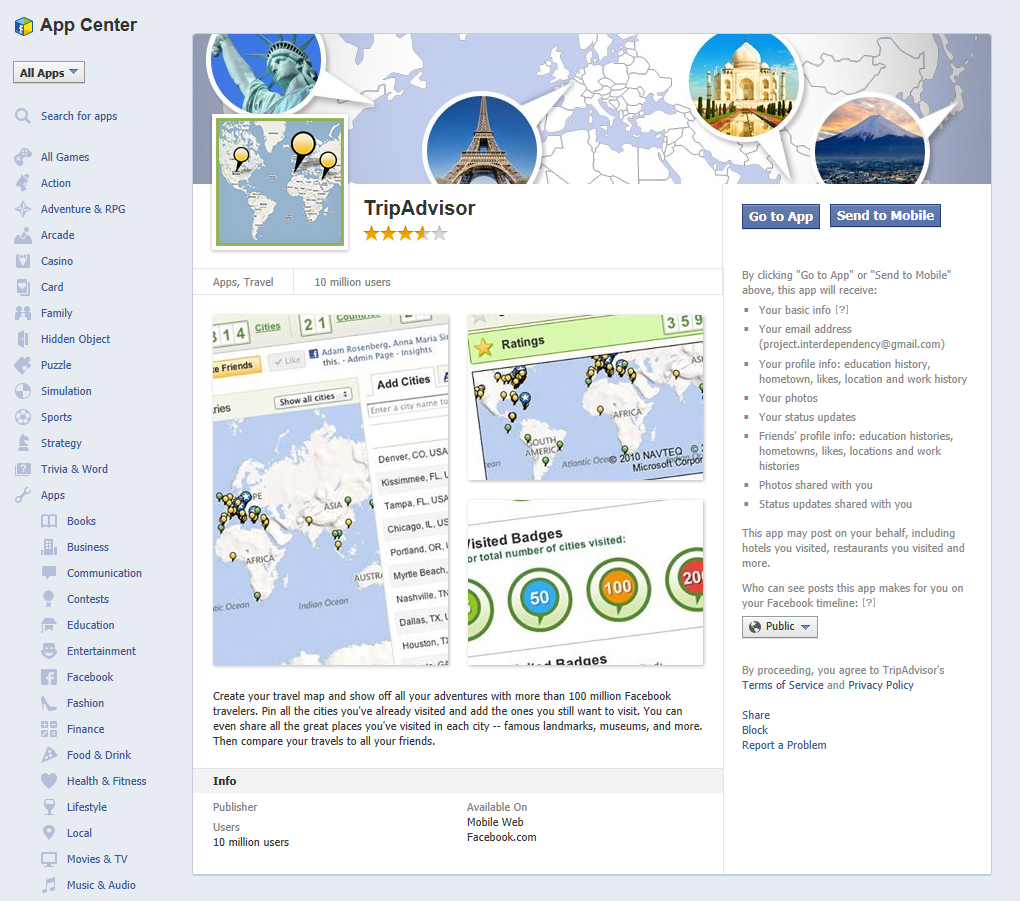
\includegraphics[width=0.8\textwidth]{tripadvisorpc.png}
\caption[At the application TripAdvisor inside Facebook's App Center]{\textbf{At the application TripAdvisor inside Facebook's App Center.} } 
\label{fig:tripadvisorpc}
\end{figure}

\begin{figure}[h!]
\centering
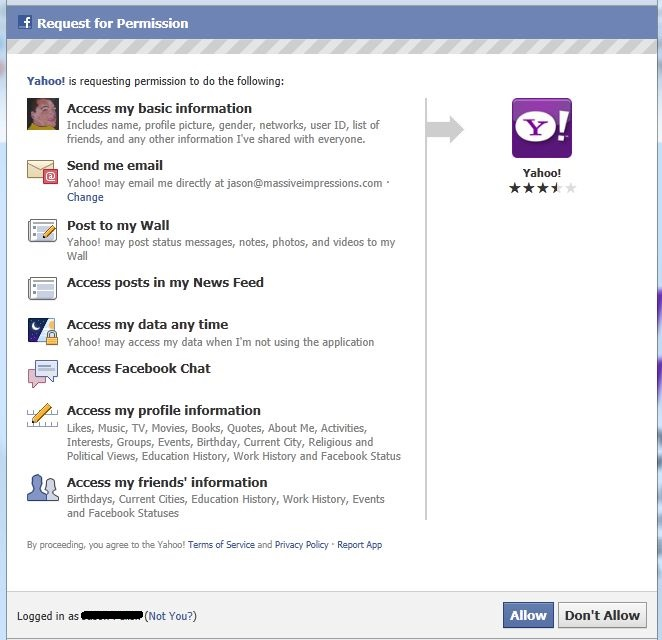
\includegraphics[width=0.8\textwidth]{permissions.jpg}
\caption[Request for permission when installing app anno 2011]{\textbf{Request for permission when installing app anno 2011.} } 
\label{fig:permissions2011}
\end{figure}

\paragraph{Installing on a mobile phone.}
The installation process looks a bit different when you install an app on the Facebook application on a mobile phone. When clicking on the application TripAdvisor in the Facebook mobile app, the user is directed to Apples App Store or Android's Play store. \fref{fig:tripa1mobil} shows the application in Android's Play Store. When TripAdviser is installed, the user can choose if he/she would like to connect with Facebook as \fref{fig:tripa2mobil} shows. It the user choose to connect with Facebook the request for permissions will appear in a pop-up window, this you can see in \fref{fig:tripa3mobil}. The user can then choose either to cancel or press OK, which means that you give your consent. 


\begin{figure}[h!]
\centering
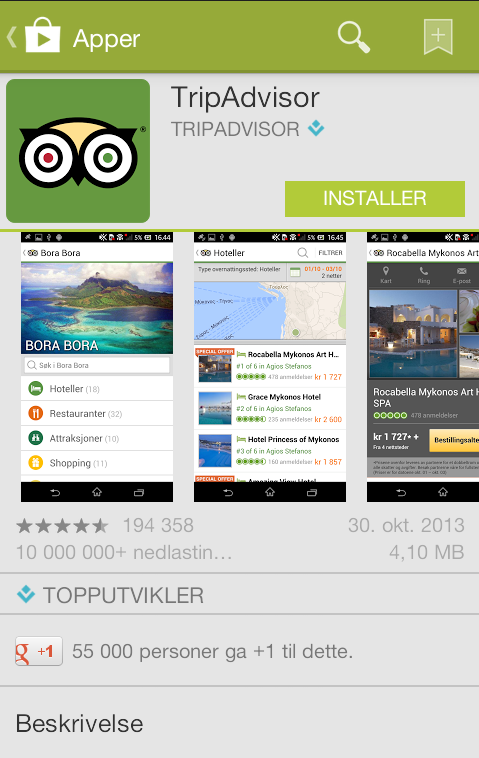
\includegraphics[width=0.5\textwidth]{tripa1mobil.png}
\caption[Installation page for TripAdvisor]{\textbf{Installation page for TripAdvisor.} This figure shows the installation page for TripAdvisor in Android's Play Store.} 
\label{fig:tripa1mobil}
\end{figure}

\begin{figure}[h!]
\centering
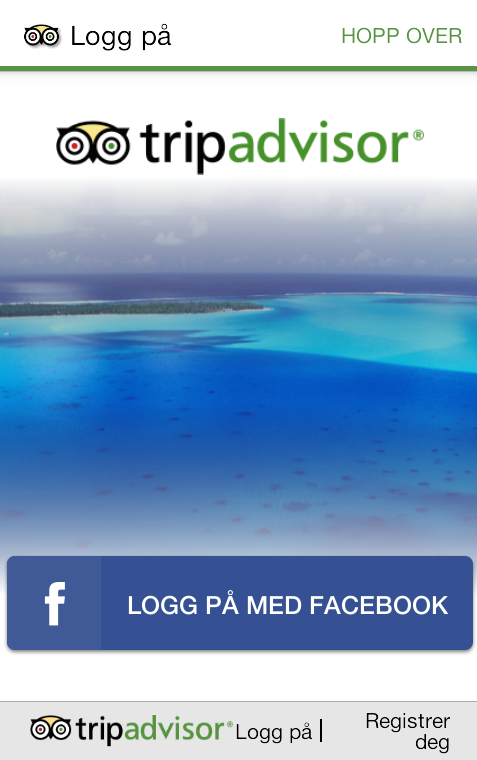
\includegraphics[width=0.5\textwidth]{tripa2mobil.png}
\caption[The page where you choose "Log in with Facebook"]{\textbf{The page where you can choose "Log in with Facebook".} On this page you can choose whether or not you want to log in with Facebook. If you choose to log in with Facebook you are redirected to the page shown in \fref{fig:tripa3mobil}.} 
\label{fig:tripa2mobil}
\end{figure}

\begin{figure}[h!]
\centering
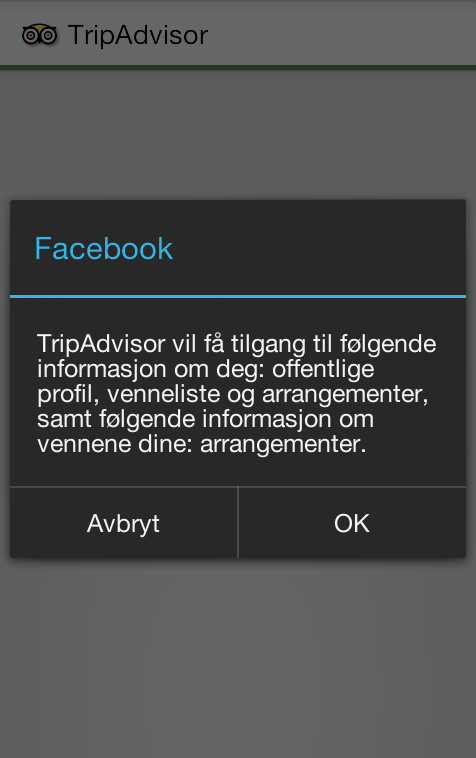
\includegraphics[width=0.5\textwidth]{tripa3mobil.png}
\caption[Facebook's request for permissions on mobile phone]{\textbf{Facebook's request for permissions on mobile phone} This figure shows the page where Facebook states what permissions they are requesting before you can start using the app. Here you can choose to either cancel or press OK.} 
\label{fig:tripa3mobil}
\end{figure}

%Launches app center
%utviklingen utseende
%installere app på web og mobil


\subsection{Beacon}
\paragraph{}
At the end of 2007 Facebook launched the feature Beacon. Beacon was created to help users easily share information from other websites with their Facebook friends \cite{BeaconWebsites}. Beacon was a key part of the Facebook Ads system. The aim was to connect businesses and users and create a more targeted advertising towards the users. 

When Beacon was launched it had 44 partner sites, among these were Live Nation, fandango.com, Trip Advisor, STA travel, eBay, the Knot and Zappos.com. According to the Facebook announcement \cite{BeaconWebsites} these websites could determine which actions was most relevant and appropriate for a user to share on Facebook. This could be anything from watching a video, a new high score on an online game, posting an item for sale or completing a online purchase. When a user, that is logged on to Facebook, enters a website that is part of Beacon, they will receive a message asking whether they would like to share their actions on Facebook. If a users agrees, the users actions on that page will be shown in their news feed or mini feed and shared with their friends.  

Beacon received a lot of attention and privacy concerns. Some websites posted to Facebook without asking the users if they want to share the information first. Beacon is a very short piece of code provided by Facebook. The participating websites implement this code on the actions that they would like people to share. An example described in \cite{beaconMarketsPerspective} is with the blog page TypePad. The user have the opportunity to chose whether Beacon should be turned on or not. When creating a post and publishing it the user receives a small pop-up window in the lower right corner stating that you are now sharing this information with Facebook. The pop-up allow you to decline, but here you have to be quick, the window is not visible for long. When entering Facebook a message is shown at the top of the users wall. Telling the users that a website have shared information with Facebook. You then have the opportunity to go through and select whether that website is allowed to share at all, to just friends or to the public.  

But not all websites have created an option for the users to choose for themselves whether or not to opt-in. And pushes to Facebook without notifying the users or lets the users select themselves that they want to share it. An much used example of this is a man buying an diamond engagement ring online \cite{ring}. Within hours he starts receiving congratulations from friends and family. The website had posted the purchase on the guys public Facebook page, including a link to the purchase and the price. All his friends received an notification, including his coming fiancée. So much for the surprise engagement. There are several similar stories.  
This is unfortunate for the users, but also for the companies using Beacon, it puts them in a negative light. Beacon could have been a great asset for different companies, and a great way for them to broadcast themselves. 

Another problem is that Beacon only checked that someone was logged on Facebook. When several people use one computer it could create problems, since Beacon was machine specific. One family member, the mother, could be logged on while her 10 year old son plays an online game, and manages to make a new high score. This high score will then be posted in the News Feed on the mothers Facebook profile, and shown to the mothers friends. This is not very fortunate for the mother. Beacon only checks that there is a valid Facebook cookie on the machine and then pushes the content to that Facebook user, without any validation. 

In a blog post, Mark Zuckerberg apologized for the way the feature was created and for the handling of the complaints in hindsight \cite{Beacon}. Zuckerburg explains that one of the problems with making the system opt-out, was that if a Facebook user forgot to declilne something Beacon still went ahead and posted and shared with the users friends. Further he explains that it took them too long from they started receiving complaints to they were able to decide on a solution to the issues. Facebook released features that gave the user more control. And the users got the ability to turn off Beacon completely.  In addition Facebook promised their users that they did not save the information Facebook received from the participating websites when the user had chosen to not use Beacon. 

All of beacons issues resulted in a lawsuit against Facebook, and some of the participating companies. The lawsuit resulted in a settlement, where Facebook agreed to shut down the feature and gave \$9,5 million to found a new non-profit foundation that would work with online privacy, security and safety \cite{lawsuitB}. Beacon was shut down in September 2009. Beacon is mentioned as one of the darkest marks in the history of social networks.

\subsection{Facebook Connect - "Log in with Facebook"}
From may 2008 users had the ability to connect and log in to other web pages via Facebook, "log in with Facebook". The users are allowed to connect their Facebook identity, friends, and privacy to any website supporting this feature. This was Facebook's first attempt to allow access to user data from Facebook outside of Facebook itself. The important features of Facebook Connect are stated in \tref{tab:connect}.

\begin{center}
\begin{table}[!ht]
\caption{\label{tab:connect}Facebook Connect Features \cite{connect, connect2}.}
    \begin{tabular}{ | l | p{9cm} |}
    \hline
    \textbf{Feature} & \textbf{Description} \\ 
    \hline
    Trusted Authentication & Authentication when users connect their account to a third party. During the user's experience the developer could at any time like to add additional social context. These activities need authentication from the user. In other words, the user have total control over the permissions that are granted. \\ 
    \hline
    Real Identity &  The users can port information linked to their real identity with them on the web to a third party website. This information includes basic profile information, profile picture, name, friends, photos, events, groups etc. \\ 
    \hline
    Friends Access & As mentioned, the users take their friends with them to third party sites. This makes it possible for the developers to add social context to the sites. You will also get notified if some of your friends already have an account on the site.\\
    \hline
    Dynamic Privacy & When the users move around from one place on the web to another, they always bring their privacy settings with them. This is done so one can be sure that their information and privacy settings are updated at any time. In other words, when you update your privacy settings on Facebook, they will automatically be updated on third party sites.\\
	\hline
    \end{tabular}
   \end{table}
\end{center}


\subsection{Places}
The feature Places was launched in the United States August 2010, and later in te rest of the world, this enabled the users "check in" using their mobile device \cite{checkIn}. This feature enables the users to share a place that they really like with their friends. This can be a cafè, a new restaurant, a concert or maybe a nice hiking trail. Have you ever been to a concert and found out afterwards that several of your friends also where there? This is what the feature places solves for you. You can for example check in to the concert, and see who else is there or see who of your friends is close by. After you have checked in at a place, your check-in will appear in your friends News Feed. It is possible to tag the friends you are with. The user are in control of what is shared and who it is shared with. A user chooses weather or not they want to share the location they are at. If a user is tagged in a check-in, they will will always be notified. The default audience is "friends", unless the users chooses to share differently, for example with "everyone", or a more restrict option, just specific friends. 

This feature is also used with third-party applications, like Tripadvisor or other travel planning applications. They collect your check-ins to generate a mat that shows where you have been in the world. So if you are planning on going to Paris you can see who else has been there and also at what places, restaurants etc., they have checked in to. 
When you write a post on Facebook you can decide if you would like to add a location to the post. And when creating the post you also decide the audience. On the mobile phone it is a little different. Here the location setting is located in the phone settings and not in the Facebook settings on the phone. The places setting on the phone can get your location by using Wi-Fi, mobile network or GPS signals. if one of these are turned on, the users location will appear on chat messages. When a user writes a post and wants to add a locations, the phone asks the user to turn on GPS, this to get a more accurate location. If the users desires not to turn it on he/she can write in a location, for example "Oslo", and Facebook will suggest places. A feature on the Facebooks mobile application is "places nearby". Here the user can see what places that is close to their current location, and what friends that have liked the page and rating from other users. This is shown in \fref{fig:nearby} and \fref{fig:places}. A user also have the ability to add locations to photos that they post themselves or that others have posted. 

\begin{figure}[h!]
\centering
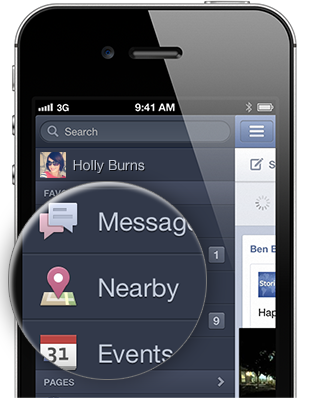
\includegraphics[width=0.3\textwidth]{nearby.png}
\caption[Nearby function on Facebook mobile]{\textbf{Nearby function on Facebook mobile.}  Where in the mobile application of Facebook to find the "places nearby"-feature.  } 
\label{fig:nearby}
\end{figure}

\begin{figure}[h!]
\centering
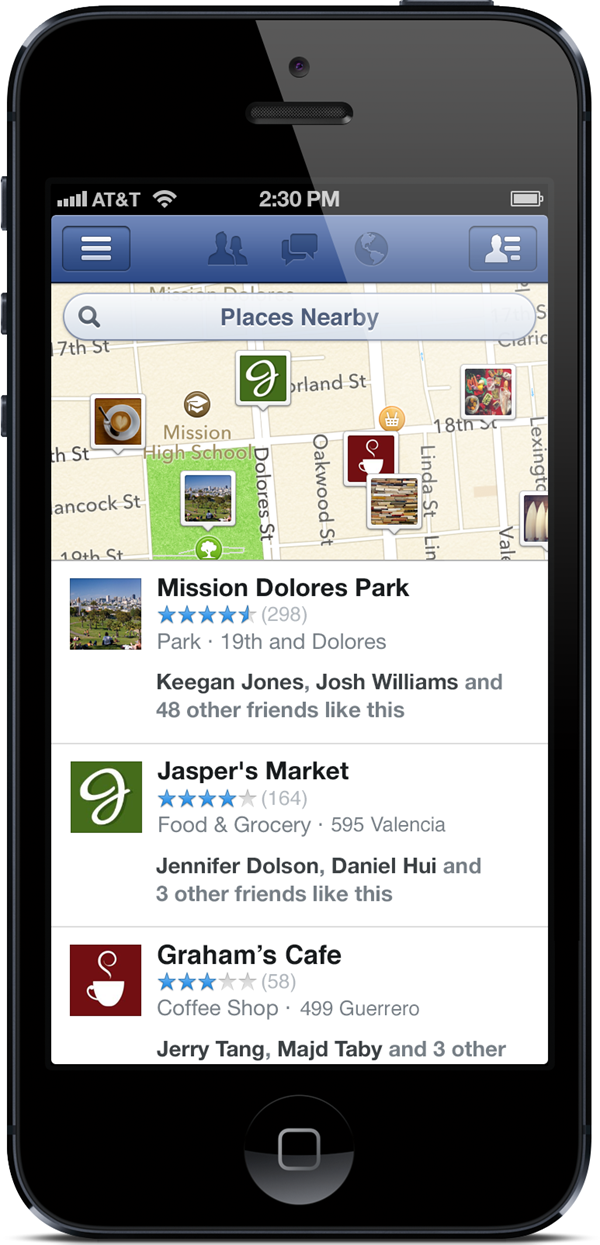
\includegraphics[width=0.3\textwidth]{places.png}
\caption [Places nearby feature]{\textbf{Places nearby feature.} Displaying the screen where the users can see what kind of places that is close to their current location. It shows which friends like the certain place or has checked in there.} 
\label{fig:places}
\end{figure}

\subsection{Timeline}
As mentioned in section \ref{sec:facebookhistory} in Chapter 1, the Facebook timeline was introduced in December 2011 \cite{EvolutionOfFacebook}. This feature made the entire history of the users visible: your posts, posts by others, likes, photos, links, pages liked, comments and other things that you have shared on Facebook. The timeline showed much more than the old profile did, and it was far more visual \cite{timeline}. On the top of your timeline it is room for a big photo. This photo is called a \emph{cover photo}. Cover photos are publicly available, and it is not possible to change the settings for them. You can of course choose which photo you want as your cover photo, or just choose not to have a photo there at all. When scrolling down your timeline , you'll see photos, posts etc. and different events in your life in order of when they happend in time \cite{timeline}. You can look at it as the story of your life. You get the opportunity to "go back in time" and fill in the blanks. If you want to emphasize, for example an event or a photo, you can highlight it with a star, or on the other hand, if you want to hide something from the timeline you can also do so. 

\paragraph{Privacy concerns regarding Facebook timeline}
When timeline was introduced many people became overwhelmed by the changes, and felt they lost control over their privacy. When you agreed to start using timeline, you got a certain period of time to review and edit your timeline before making it public. This gave the users the opportunity to clean up their timeline before everyone else could view the content of it. Cleaning up the timeline can be done using something called the "Activity Log" \cite{activitylog}, which is shown in \fref{fig:activitylog}. The activity log is basically a list over everything ever done in connection with you on Facebook, either done by you or by others. The activity log also makes it easy to view and change the audience for the different "activities". If you are an active user of Facebook, reviewing the whole activity log can be very time consuming. 

\begin{figure}[h!]
\centering
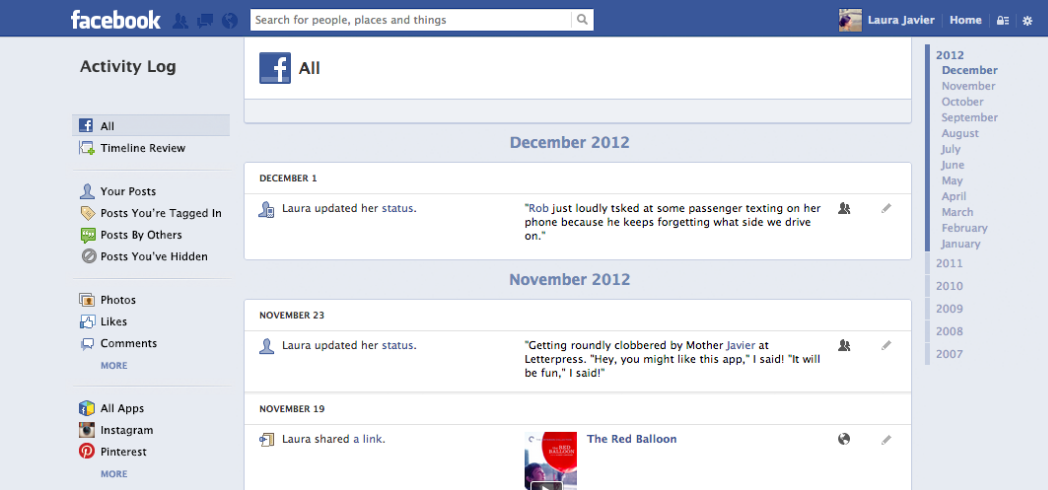
\includegraphics[width=1\textwidth]{activity_log.png}
\caption [Example of an activity log on Facebook.]{\textbf{Example of an activity log on Facebook}. On the left side you see types of content. If you want to view for example "Posts by others" you can do so by clicking on it. To the right you see a list of the years and months. You can click on which year or month you want, and review the activity from that year/month \cite{activitylog}} 
\label{fig:activitylog}
\end{figure}

\paragraph{}
The introduction of timeline was not in itself a privacy breach since you had, and still have, the opportunity to decide what you want to be visible on it, and what you want to hide. On the other hand, there are people who are extra exposed when Facebook introduced new major changes, like the timeline. Lets refer back to section \ref{sec:relatedwork_facebookprivacy} in Chapter \ref{chp:relatedwork}, where we highlighted some of the findings from the survey addressed in the paper "Facebook privacy settings; Who cares?" by danah boyd and Eszter Hargittai \cite{whocares}. boyd and Hargittai concluded their paper, based on their survey and findings, that experience and Internet skill is important to take into account in regard to how people handle their privacy settings on Facebook. Since familiarity with technology plays a role in how people handle their Facebook privacy settings, one can assume that the least skilled people get more exposed when Facebook changes the outline of the default privacy settings. 
This can be seen in the context with the introduction of the timeline. The least skilled users of Facebook that perhaps do not know how to change their privacy settings, probably was left extra exposed when the timeline was introduced and their timeline may have shown, and may still show, more than they actually would prefer. 

There also exits privacy settings connected to you timeline under "Timeline and tagging" in your settings on Facebook. You can regulate who can add things to your timeline, and who can see things on your timeline. Under "Privacy" you can also regulate who can see your future posts. 

\subsection{Graph Search}
Graph Search is a semantic search engine introduced in a beta version by Facebook in March 2013. During the summer 2013 the Graph Search became available for everyone using Facebook with US English language \cite{graphsearchnet}. The old search bar at the top of the page is replaced with a larger search bar, Graph Search \cite{graphsearchfb}. The Graph Search enables the users to search using natural language queries, and not just search using keywords. In addition to this the search results will be based on both relationships and content \citep{graphsearchnet}. Two examples are "Photos of 'friend's name' are tagged in" and "Restaurants in Oslo, Norway visited by my friends". The basic idea is that the users are given the possibility to search Facebook for different stuff (photos, people, places etc.) in a specific subset, specifying the queries \cite{graphsearchew}. To emphasize how specific the search can be, we will provide you with an example. Let us say you met someone at a party and the only thing you know about the person is the name, where the person goes to school and you know that the person is a friend of one of your Facebook friends, you can write a query which reads as follows: \textit{"People named 'name of the person' that are friends with 'name of the common acquaintance' and who go to 'name of schoool'"}. Off course this may not give the outcome you wanted, if the person for example have not given any information about where he/she goes to school on Facebook. Just having the opportunity to perform such queries gives the user more power, and makes it easier to connect to new people. 

Zuckerberg says that Graph Search is centered around "making new connections", because the feature makes it easier to make new connections \cite{graphsearchew}. Facebook emphasizes that the purpose of Graph Search is not to replace traditional web search. The Graph Search concerns, on the other hand, the filtering of all photos and all connections on Facebook. Since Facebook is the largest online social network in the work, it is \textit{not just a few} photos and connections available, but over 240 billion photos and over 1 trillion connections. The choices you have made in your settings determine what friends and others can see when they conduct a Graph Search \cite{graphsearchtips}. If a photo is set to "Only me" no one else can find it in the search, it it is set to "Friends" friends can find it in their search, and if it is set to "Public" anyone who searches for it can find it. Graph Search is in other words a good tool for viewing as many photos as you are allowed to view of people who are not your Facebook friends. The photos of you that are public will come up in a Graph Search regardless of how you have set your privacy settings. As long as someone has posted a photo of you as public, the entire Facebook can find and view this photo via Graph Search. So if you are interested in viewing pictures of a specific person who is not your friend on Facebook, it is not necessary to start digging through numerous albums and so on, but just do this with a quick search. 

A limited group of people got access to Graph Search in January 2013. During a introductory press conference, Mark Zuckerberg stated that Graph Search was in it's early stages, and that it will take years to complete it. He said: "Graph Search is a really big project, and it's going to take years and years to index the whole map of the graph". After the introduction of Graph Search, many questions was brought up about the privacy issues regarding it. One of the issues brought up was that the tool makes it easier for people to retrieve information and photos about other people who do not want this content to be available and seen. The fact is that people only get to view content they already could view, but it makes it much easier to find this content. Facebook  assured that Graph Search does not affect the privacy of minors. They stated that identifying information about those between the ages of 13 and 17 would only be shared with friends of friends of that minor \cite{graphsearchcw}. 

Graph search is for the time being still only available for users using US English language on their Facebook, but is a work in progress like mentioned before. Facebook has stated that further work on the feature deals with searching across posts, comments and mobile \cite{graphsearchcw}. 


\subsection{Facebook Removes Search Privacy Setting}
Facebook announced October 11 that they will remove the setting that has made it possible for Facebooks users to hide from the ability to be looked up on the Internet\cite{searchSetting}. It was only the users that have not used the setting "who can look up my timeline by name" in December by last year that was affected by the change. Facebook explains the removal of the feature by it being outdated, and that there are several others ways to find a persons time line. They argue that it can be confusing for the user when they try to look up someone and do not find them. Mark Zuckerberg said that a users should do things they want to keep secret.

(sånn jeg ser det så er det jo fult mulig å søke opp hvem som helt på facebook sin egen søkefunksjon, det betyr jo ikke ta jeg ønsker å være søkbar på google. 


\section{Zuckerberg's Thoughts}

\paragraph{}
Zuckerberg ones said this about Facebook in a one of his meetings: "I mean, one way to look at the goal of the site is to increase people’s understanding of the world around them, to increase their information supply," he said. "The way you do that best is by having people share as much information as they are comfortable with. The way you make people comfortable is by giving them control over exactly who can see what" \cite{MeMedia}.

\paragraph{}
This comment from Zuckerberg brings out his thoughts around the privacy issues. He wants the users of Facebook to be comfortable with sharing information, and give them this confidence by giving them control. In general the privacy settings and restrictions that Facebook has have protected the users. They can easily change the setting and decide who can see what. Zuckerburg firmly means that you should not post comments or pictures of things you do not want anybody else to see. And if a user does so, the user has to take the blame for it, not Facebook. Zuckerberg was once asked about pictures put on Facebook of students drinking at an East Coast college, which led to some students being expelled. His answer to this question was: "First of all, it's pretty stupid if you put up pictures of you doing drugs on Facebook. I think that that's just sort of the deviant behavior on the very far end of the distribution. I bet that those kids do not post pictures of them doing drugs on Facebook anymore." He added that he meant this was a "pretty shitty way to learn that" \cite{MeMedia}.

\paragraph{}
Mark Zuckerberg wrote this in a letter to possible investors \cite{LetterToInvestors}; \textit{Facebook was not originally created to be a company. It was built to accomplish a social mission - to make the world more open and connected.} \textit{People sharing more - even if just with their close friends or families - creates a more open culture and leads to a better understanding of the lives and perspectives of others. We believe that this creates a greater number of stronger relationships between people, and that it helps people get exposed to a greater number of diverse perspectives.}
